% ─────────────────────────────────────────────────────────────────
\section{Ablation Studies}
\label{sec:ablation}
% ─────────────────────────────────────────────────────────────────

\subsection{Feature Mode Ablation}
\label{sec:ablation:features}

We train five HierGIN-h512 models that differ only in which subset of the
8D feature vector is used, keeping all other hyperparameters fixed
(Table~\ref{tab:feature_modes}).

\begin{table}[h]
  \centering
  \caption{Feature mode definitions. Dimension counts the entries of
           $\mathbf{x}_i$ fed to the node GIN. All 8D indices:
           [0]=Potential\_norm, [1]=NormPot\_norm, [2--4]=$(n_x,n_y,n_z)$,
           [5--7]=$(x,y,z)_\text{ssl}$.}
  \label{tab:feature_modes}
  \begin{tabular}{lclp{5.5cm}}
    \toprule
    \textbf{Name} & \textbf{Dim} & \textbf{Indices} & \textbf{Contents} \\
    \midrule
    \texttt{coords\_potential}  & 4  & [0,5,6,7] & Potential + xyz \\
    \texttt{coords\_normals}    & 6  & [2,3,4,5,6,7] & Normals + xyz \\
    \texttt{all\_no\_normpot}   & 7  & [0,2,3,4,5,6,7] & Potential + Normals + xyz \\
    \texttt{all}                & 8  & [0,1,2,3,4,5,6,7] & All features \\
    \texttt{all\_no\_pot}       & 7  & [1,2,3,4,5,6,7] & NormPot + Normals + xyz \\
    \bottomrule
  \end{tabular}
\end{table}

Table~\ref{tab:ablation_metrics} reports the test metrics computed with the
proper evaluation protocol: macro-F1, balanced accuracy, and weighted F1 are
computed over the 88 classes with at least one test protein.

\begin{table}[h]
  \centering
  \caption{Feature ablation test metrics (HierGIN h=512, eval over 88 classes).
           Best values in bold.}
  \label{tab:ablation_metrics}
  \begin{tabular}{lrrrr}
    \toprule
    \textbf{Feature config} & \textbf{Accuracy} & \textbf{Bal.\ Acc.} & \textbf{Macro-F1} & \textbf{Wtd-F1} \\
    \midrule
    \textbf{8D (all)}        & \textbf{0.8533} & \textbf{0.7997} & \textbf{0.7983} & \textbf{0.8532} \\
    7D (no NormPot)          & 0.8486 & 0.7966 & 0.7896 & 0.8479 \\
    4D (xyz + Potential)     & 0.8447 & 0.7955 & 0.7839 & 0.8434 \\
    7D (no Potential)        & 0.8079 & 0.6813 & 0.6802 & 0.7993 \\
    6D (xyz + Normals)       & 0.7828 & 0.6123 & 0.6190 & 0.7602 \\
    \bottomrule
  \end{tabular}
\end{table}

\begin{figure}[h]
  \centering
  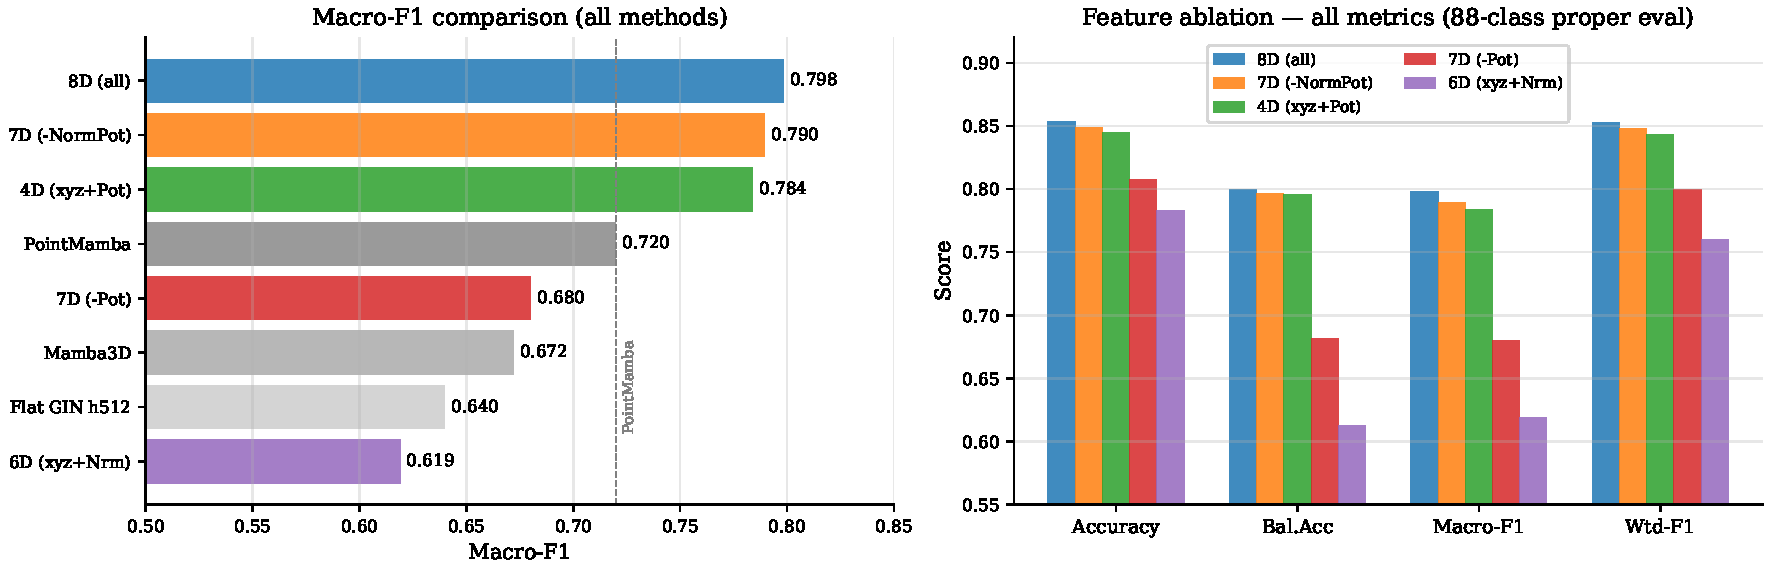
\includegraphics[width=\linewidth]{figures/feature_ablation_summary.pdf}
  \caption{Left: macro-F1 of all feature configurations and external methods.
           Right: full metric comparison across the five ablation configs.
           The 8D model outperforms all single-feature subsets.}
  \label{fig:ablation_summary}
\end{figure}

\paragraph{Findings.}

\begin{enumerate}
  \item \textbf{Electrostatic potential is irreplaceable.}
        Removing \textit{Potential} (7D-no-Pot vs.\ 8D) costs $-$11.8\,pp
        macro-F1.
        This matches the KS and SW analyses: Potential is the dominant
        discriminating signal for all separable pairs.

  \item \textbf{NormalPotential provides a modest global gain.}
        The 4D model (xyz + Potential only) vs.\ 8D loses $-$1.4\,pp
        macro-F1.
        However, removing NormalPotential (7D-no-NP) causes a $-$14\,pp F1
        drop specifically for class\,61 (see Table~\ref{tab:per_class_f1}),
        suggesting that NormalPotential encodes information critical to
        distinguishing the hardest pairs.

  \item \textbf{Normals contribute but are not sufficient alone.}
        The 6D model (xyz + normals, no potential) achieves only 0.619
        macro-F1, confirming that normals alone cannot compensate for the
        loss of electrostatic potential.

  \item \textbf{8D is globally optimal.}
        Adding all features ($+$NormPot$+$Normals over 4D) improves
        macro-F1 by $+$1.4\,pp while slightly improving balanced accuracy.
\end{enumerate}

\begin{figure}[h]
  \centering
  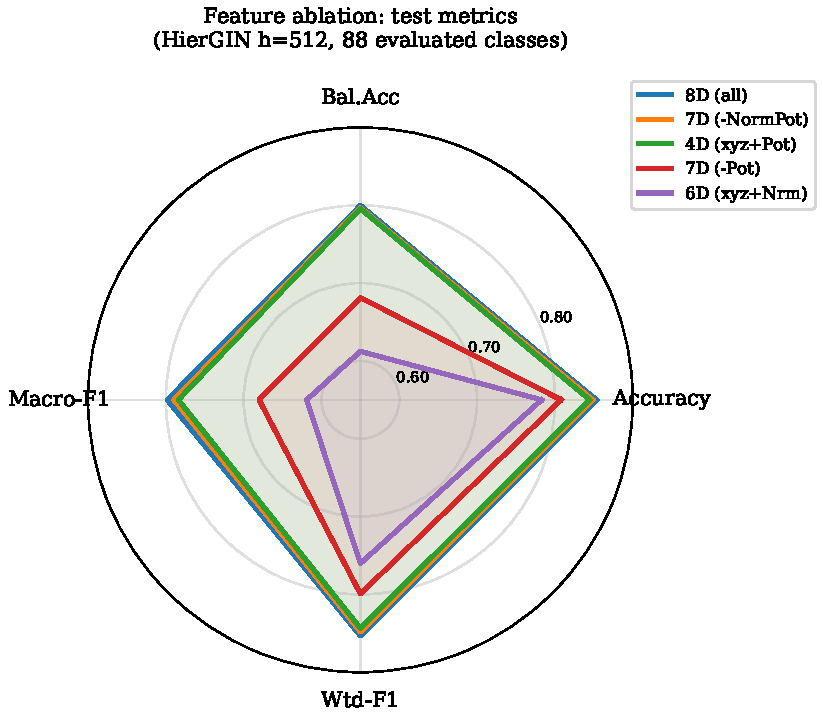
\includegraphics[width=\linewidth]{figures/feature_ablation_radar.pdf}
  \caption{Radar chart: four metrics across five feature configurations.
           The 8D polygon (blue) is uniformly larger; the 6D and 7D-no-Pot
           polygons collapse on the balanced accuracy axis,
           reflecting their inability to handle rare classes.}
  \label{fig:radar}
\end{figure}

\begin{table}[h]
  \centering
  \caption{Per-class F1 on hard/confusable classes for each feature configuration.}
  \label{tab:per_class_f1}
  \begin{tabular}{lrrrrrrr}
    \toprule
    \textbf{Config} & \textbf{cls\,61} & \textbf{cls\,90} & \textbf{cls\,70} & \textbf{cls\,56} & \textbf{cls\,86} & \textbf{cls\,14} & \textbf{cls\,80} \\
    \midrule
    8D (all)         & 0.576 & 0.850 & 0.532 & 0.775 & 0.667 & 0.729 & 0.174 \\
    7D (no NormPot)  & 0.474 & 0.850 & 0.571 & 0.760 & 0.690 & 0.690 & 0.333 \\
    4D (xyz+Pot)     & 0.435 & 0.832 & 0.509 & 0.726 & 0.643 & 0.754 & 0.091 \\
    7D (no Pot)      & 0.321 & 0.870 & 0.392 & 0.708 & 0.529 & 0.634 & 0.174 \\
    6D (xyz+Nrm)     & 0.300 & 0.860 & 0.203 & 0.743 & 0.486 & 0.560 & 0.000 \\
    \bottomrule
  \end{tabular}
\end{table}

Figure~\ref{fig:per_class} visualises these per-class results.

\begin{figure}[h]
  \centering
  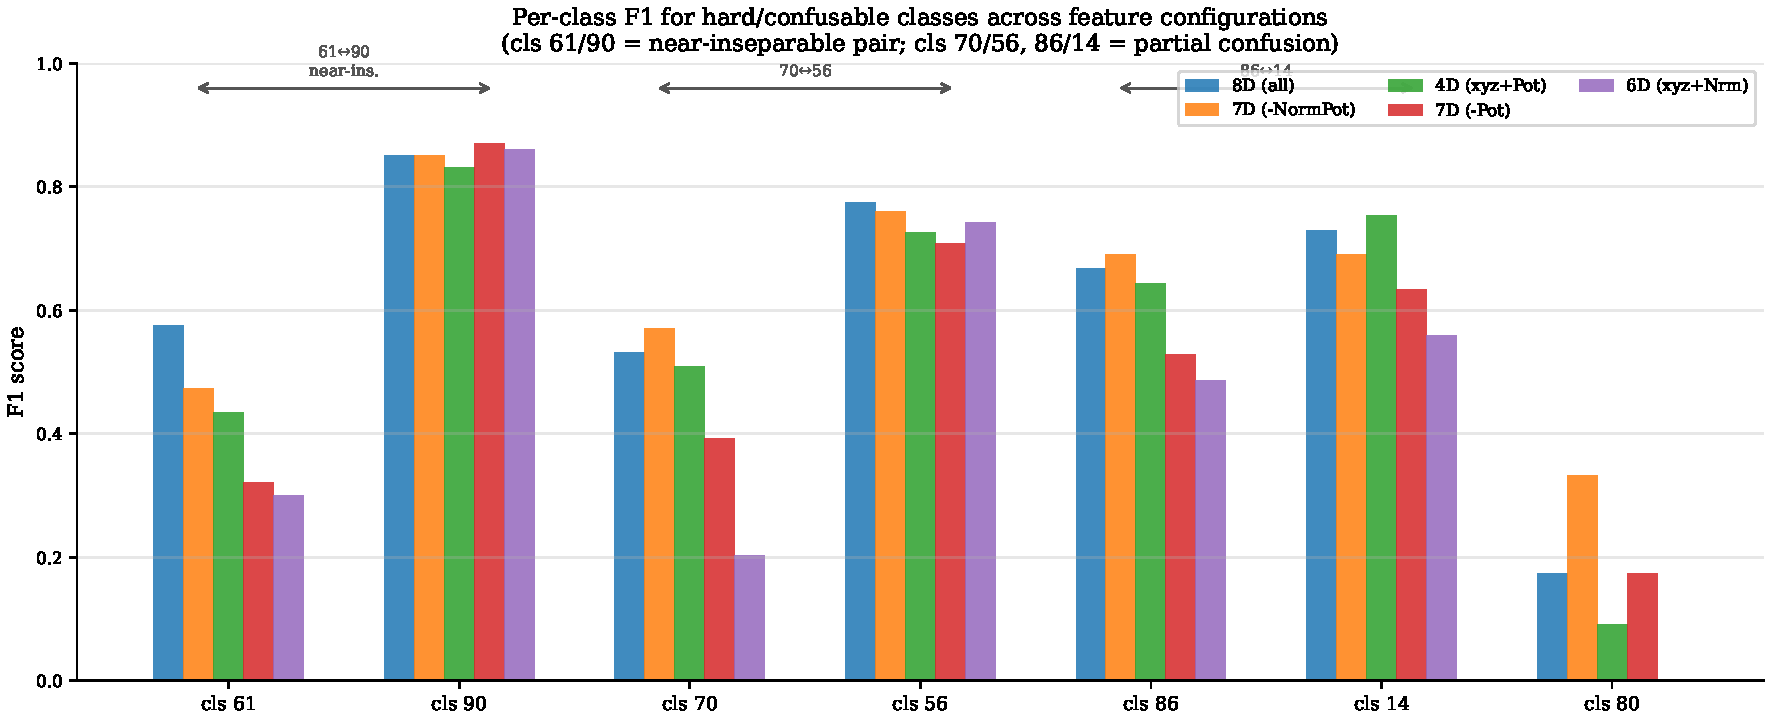
\includegraphics[width=\linewidth]{figures/per_class_f1_hard.pdf}
  \caption{Per-class F1 for the seven hardest classes across all five feature
           configurations.
           Class\,61 shows the largest variance across configurations,
           benefitting most from NormalPotential.
           Class\,80 is effectively unlearnable with 6D features.}
  \label{fig:per_class}
\end{figure}

\begin{figure}[h]
  \centering
  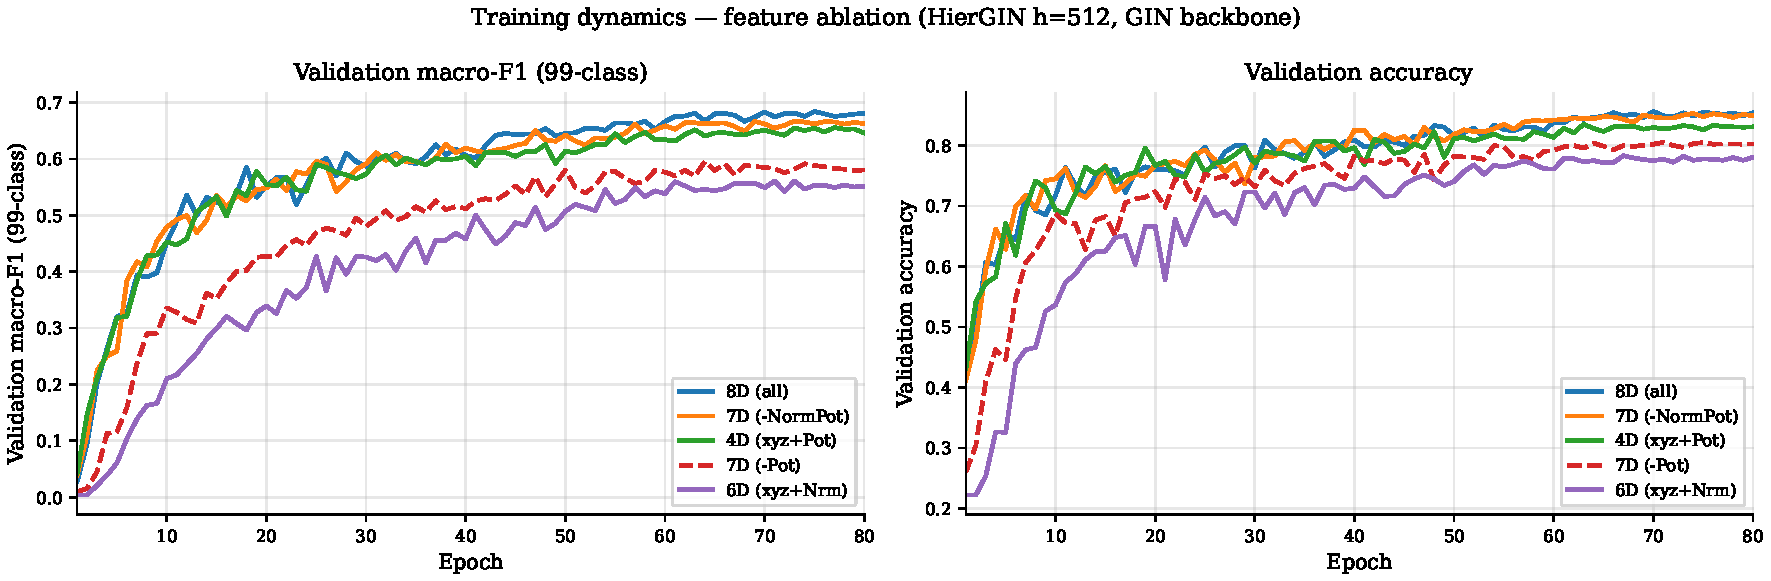
\includegraphics[width=\linewidth]{figures/training_curves_features.pdf}
  \caption{Validation training dynamics for the five feature ablation runs.
           Dashed lines: configurations without Potential (7D-no-Pot, 6D) converge
           to a much lower ceiling.}
  \label{fig:training_curves_feat}
\end{figure}

\subsection{Patch Count Ablation}

We evaluate $k \in \{8, 32, 64, 128\}$ patches under the 4D feature
configuration with all other settings fixed.

\begin{center}
  \begin{tabular}{crr}
    \toprule
    \textbf{Patches $k$} & \textbf{Best val F1} & \textbf{Relative} \\
    \midrule
    8   & 0.570 & $-$9.4\,pp \\
    32  & 0.618 & $-$4.6\,pp \\
    \textbf{64}  & \textbf{0.655} & baseline \\
    128 & 0.643 & $-$1.2\,pp \\
    \bottomrule
  \end{tabular}
\end{center}

$k = 64$ provides the best trade-off: too few patches ($k=8$) loses too much
spatial resolution, while $k=128$ provides marginal improvement at higher
computational cost.

\subsection{Hidden Dimension}

Hidden dimension $h=512$ outperforms $h=256$ by approximately $+$2\,pp
macro-F1 in all tested configurations.
Increasing to $h=1024$ produced no further improvement and significantly
increased GPU memory usage.

\subsection{Node GIN Depth}

Three node GIN layers ($L_n = 3$) outperform both $L_n = 2$ ($-$0.8\,pp) and
$L_n = 6$ ($-$1.5\,pp), suggesting slight overfitting with deeper node
stacks.

\subsection{LR Schedule}

Cosine annealing with warmup outperforms step decay ($-$0.5\,pp) and no
scheduling ($-$1.8\,pp) on validation macro-F1.

\subsection{Random Walk Positional Encoding}

Adding RWPE with $k_\text{rw} = 16$ provides a marginal $+$0.3\,pp gain on
validation F1 but adds 16 dimensions to each node feature vector and
increases memory usage.
The best test-set run (HierGIN-8D) uses no RWPE ($k_\text{rw} = 0$) to keep
the model compact.

\subsection{Patch-level Scalar Re-injection}
\label{sec:ablation:patch_inject}

\paragraph{Motivation.}
The attention pooling step aggregates node embeddings into 512-dimensional
patch vectors; from that point on, the patch GNN operates entirely in the
learned embedding space.
We hypothesised that the raw electrostatic signal (Potential, NormalPotential)
may be ``washed out'' during pooling and could be recovered by explicitly
re-injecting patch-mean raw scalars between the two patch GNN layers:

\begin{equation}
  \mathbf{p}_c^{(\ell)} \leftarrow
  W \!\left[\mathbf{p}_c^{(\ell)} \;\Big\|\; \bar{\mathbf{s}}_c\right],
  \quad
  \bar{\mathbf{s}}_c = \frac{1}{|\mathcal{P}_c|}
    \sum_{i \in \mathcal{P}_c} \mathbf{s}_i,
\end{equation}

where $\mathbf{s}_i$ are the raw scalar features of node $i$ and $W$ is a
learned projection.

\paragraph{Experiments.}
We test two injection variants on the 14D (global norm) feature set, with all
other hyperparameters matching the best baseline run:
\begin{itemize}
  \item \textbf{2-feat}: inject patch-mean of [Potential, NormalPotential] only.
  \item \textbf{8-feat}: inject patch-mean of all signal scalars
        ([Potential, NormalPotential] $+$ the 6 geometric features),
        skipping normals and coordinates.
\end{itemize}

\begin{center}
  \begin{tabular}{lrr}
    \toprule
    \textbf{Configuration} & \textbf{Macro-F1 (88)} & \textbf{vs.\ baseline} \\
    \midrule
    HierGIN-14D (global norm, no injection) & 0.808 & --- \\
    + 2-feat injection (Pot, NormPot)       & 0.790 & $-$1.8\,pp \\
    + 8-feat injection (all scalars)        & 0.778 & $-$3.0\,pp \\
    \bottomrule
  \end{tabular}
\end{center}

\paragraph{Findings.}
Both variants \emph{regress}, with more features injected causing a larger
drop.
We attribute this to two factors: (1) the attention pooling already
concentrates the electrostatic signal into the patch embeddings, so
re-injection introduces redundant and noisy supervision; (2) the linear
projection $W$ disrupts the learned patch representation by forcing it to
re-encode information it already contains.
The result rules out ``signal loss through pooling'' as an explanation for
the remaining accuracy gap.

\subsection{Rotation-Invariant Node Backbone (RI-GIN)}
\label{sec:ablation:rigin}

\paragraph{Motivation.}
Standard GIN processes node features expressed in an arbitrary global
coordinate frame, meaning that the same protein surface in different
orientations produces different embeddings.
Although the training set presumably contains proteins in varied orientations
and the model can learn to be approximately invariant by memorising
representative orientations, hard-coding rotation invariance into the
architecture eliminates this burden entirely.

\paragraph{Implementation.}
We replace the node-level GIN with the RI-GIN backbone described in
Section~\ref{sec:arch:rigin}.
The patch-level GIN and all other components remain unchanged.
The model is trained under two feature modes:
(i)~\textbf{8D (all)} on the standard SSL graph dataset;
(ii)~\textbf{14D (geom, global norm)} on the geometry-enriched dataset.

\paragraph{Results.}
Both runs are currently training.
Table~\ref{tab:rigin} will be updated once training completes.

\begin{table}[h]
  \centering
  \caption{RI-GIN vs.\ standard GIN on the same feature sets (88-class eval).
           RI-GIN results pending.}
  \label{tab:rigin}
  \begin{tabular}{llrr}
    \toprule
    \textbf{Backbone} & \textbf{Features} & \textbf{Macro-F1} & \textbf{Bal.\ Acc.} \\
    \midrule
    GIN    & 8D (all)             & 0.798 & 0.800 \\
    RI-GIN & 8D (all)             & \textit{pending} & \textit{pending} \\
    \midrule
    GIN    & 14D (global norm)    & 0.808 & 0.812 \\
    RI-GIN & 14D (global norm)    & \textit{pending} & \textit{pending} \\
    \bottomrule
  \end{tabular}
\end{table}

\paragraph{Memory constraint.}
At $h = 512$ and batch size 64, the RI-GIN edge MLP materialises $\sim$750\,MB
per layer, making it impossible to run two experiments simultaneously on a
12\,GB GPU.
The 14D run is therefore launched sequentially after the 8D run completes,
with batch size reduced to 32.
